\chapter{内存管理}

\section{实验目的}
  \begin{enumerate}
    \item 了解MIPS内存映射布局
    \item 掌握使用空闲链表的管理物理内存的方法
    \item 建立页表,实现分页式虚存管理
    \item 实现内存分配和释放的函数
  \end{enumerate}

本次实验中,我们需要掌握MIPS页式内存管理机制,需要使用一些数据结构来记录内存的使用情况,并实现内存分配
和释放的相关函数,完成物理内存管理和虚拟内存管理。

\section{MMU和TLB}

首先介绍两个与内存管理有关的概念:MMU和TLB。

\begin{note}
MMU,即内存管理单元(memory‐management unit)。MMU 是 CPU 中用来管理虚拟存储器、物理存储器的
控制线路,同时也负责虚拟地址映射为物理地址,以及提供硬件机制的内存访问授权。
\end{note}

\begin{note}
TLB,即翻译后备缓冲(translation lookaside buffer, 这个全称对你理解这个术语可能不会帮多少忙)。
TLB 是将程序使用的地址(虚拟地址)翻译成物理地址(访问内存的地址)的硬件。TLB在大多数时候只能映射PC
物理内存空间的一小部分,主要是作为一个软件管理的地址翻译的缓存来使用。当一个需要的地址翻译不在TLB中时,
就会产生一个异常,而由异常处理程序来计算并装载正确的翻译。在我们之后的工作中,我们也会看到这一点。
\end{note}

\section{MIPS虚存映射布局}

32位的MIPS CPU最大寻址空间为4GB(2\^32字节),这4GB虚存空间被划分为四个部分:

\begin{enumerate}
  \item kuseg (TLB-mapped cacheable user space, 0x00000000 ~ 0x7fffffff):
  这一段是用户模式下可用的地址,大小为2G,也就是MIPS约定的用户内存空间。需要通过MMU进行虚拟地址到物理
  地址的转换。
  \item kseg0 (direct-mapped cached kernel space, 0x80000000 ~ 0x9fffffff):
  这一段是内核地址,其内存虚存地址到物理内存地址的映射转换不通过MMU,使用时只需要将地址的最高位清零
  (\& 0x7fffffff),
  这些地址就被转换为物理地址。也就是说,这段逻辑地址被连续地映射到物理内存的低端512M空间。对这段地址
  的存取都会通过高速缓存(cached)。通常在没有MMU的系统中,这段空间用于存放大多数程序和数据。对于有
  MMU 的系统,操作系统的内核会存放在这个区域。
  \item kseg1 (direct-mapped uncached kernel space, 0xa0000000 ~ 0xbfffffff):
  与kseg1类似,这段地址也是内核地址,将虚拟地址的高 3 位清零(\& 0x1fffffff),就可以转换到物理地址,
  这段逻辑地址也是被连续地映射到物理内存的低端512M空间。但是 kseg1 不使用缓存(uncached),访问速度比较慢,
  但对硬件I/O寄存器来说,也就不存在Cache一致性的问题了,这段内存通常被映射到I/O寄存器,用来实现对外设的访问。
  \item kseg2 (TLB-mapped cacheable kernel space, 0xc0000000 ~ 0xffffffff):
  这段地址只能在内核态下使用,并且需要 MMU 的转换。
\end{enumerate}

\section{内存管理与内存翻译}

  内存管理的实质是尾每个程序提供自己的内存空间。最为朴素的内存管理就是直接将物理内存分配给程序,一个萝卜一个坑。
  但从之前的叙述中,我们可以发现,MIPS系统中,使用了虚拟内存的技术。因此在我们的系统中,同时存在着两套地址,
  一套是真实的物理地址,另一套则是虚拟地址,这为我们的内存管理带来了许多内存翻译的工作。这些工作大多就是由
  前文所述的MMU来完成。
  为什么我们要这么做呢?原因有很多:
    \begin{enumerate}
      \item 隐藏与保护:因为加入了虚拟内存这一中间层,真实的物理地址对用户级程序是不可见的,它只能访问
      操作系统允许其访问的内存区域。
      \item 为程序分配连续的内存空间:利用虚拟内存,操作系统可以从物理分散的内存页中,构建连续的程序空间,
      这使得我们拥有更高的内存利用率。
      \item 扩展地址空间范围:如前文所述,通过虚拟内存,MIPS32位机拥有了4GB的寻址能力,这真的很cool。:)
      \item 使内存映射适合你的程序:在大型操作系统中,可能存在相同程序的多个副本同时运行,这时候通过内存翻译
      这一中间层,你能使他们都使用相同的程序地址,这让很多工作都简单了很多。
      \item 重定位:程序入口地址和预先声明的数据在程序编译的过程中就确定了。但通过MMU的内存翻译,我们能够让程
      序运行在内存中的任何位置。
    \end{enumerate}
  为了这些好处,我们需要付出地址翻译工作的代价。接下来我们在lab的工作中,也将一直遇到这个问题。建议各位在lab的
  过程中,不妨思考当前我们使用的这个地址究竟是物理地址还是虚拟地址,搞清楚这一点,对我们的lab和操作系统的理解都
  大有帮助。

\section{物理内存管理}

\subsection{初始化流程说明}
  在第一实验中,我们将内核加载到内存中的 kseg0 区域(0x80010000),成功启动并跳转到 init/main.c 中的
   main 函数开始运行,现在我们需要在 main 函数中调用定义在 init/init.c 中的 mips\_init() 函数,并
  进一步通过

  \begin{enumerate}
    \item \mintinline{c}|mips_detect_memory()|;
    \item \mintinline{c}|mips_vm_init()|;
    \item \mintinline{c}|page_init()|;
  \end{enumerate}

  这三个函数来实现物理内存管理的相关数据结构的初始化。

\subsection{内存控制块}

在MIPS CPU 中,地址转换以4KB 大小为单位,称为页。整个物理内存按4KB大小分成了许多页,我们大多数时候的
内存分配,也是以页为单位来进行。为了记录分配情况,我们需要使用 Page 结构体来记录一页内存的相关信息:

\begin{minted}[linenos]{c}
typedef LIST_ENTRY(Page) Page_LIST_entry_t;

struct Page {
    Page_LIST_entry_t pp_link;  /* free list link */
    u_short pp_ref;
};
\end{minted}

其中,\mintinline{c}|pp_ref| 用来记录这一物理页面的引用次数,\mintinline{c}|pp_link| 是当前节点
指向链表中下一个节点的指针,其类型为 \mintinline{c}|LIST_ENTRY(Page)| 。我们在 include/queue.h
中定义了一系列的宏函数来简化对链表的操作。请阅读这些宏函数的代码,理解它们的原理和巧妙之处。

\begin{thinking}\label{think-do_while}
我们注意到我们把宏函数的函数体写成了 \mintinline{c}|do { /* ... */ } while(0)| 的形式,而不是
仅仅写成形如
\mintinline{c}|{ /* ... */ }| 的语句块,这样的写法好处是什么?
\end{thinking}

在 include/pmap.h 中,我们使用 LIST\_HEAD 宏来定义了一个结构体类型 Page\_list ,在 mm/pmap.c
中,创建了一个该类型的变量 page\_free\_list 来以链表的形式表示所有的空闲物理内存:

\begin{minted}[linenos]{c}
LIST_HEAD(Page_list, Page);

static struct Page_list page_free_list; /* Free list of physical pages */
\end{minted}

\begin{thinking}\label{think-Struct page}
注意,我们定义的 Page 结构体只是一个信息的载体,它只代表了相应物理内存页的信息,它本身并不是物理内存页。
那我们的物理内存页究竟在哪呢?Page 结构体又是通过怎样的方式找到它代表的物理内存页的地址呢?
请你阅读 include/pmap.h 与 mm/pmap.c 中相关代码,给出你的想法。
\end{thinking}

\subsection{内存分配和释放}

首先,我们需要注意在 mm/pmap.c 中定义的与内存相关的全局变量:

\begin{minted}[linenos]{c}
u_long maxpa;            /* Maximum physical address */
u_long npage;            /* Amount of memory(in pages) */
u_long basemem;          /* Amount of base memory(in bytes) */
u_long extmem;           /* Amount of extended memory(in bytes) */
\end{minted}

\begin{exercise}
我们需要在 mips\_detect\_memory() 函数中初始化这几个全局变量,以确定内核可用的物理内存的大小和范围。
根据代码注释中的提示,完成 mips\_detect\_memory() 函数。
\end{exercise}

在操作系统刚刚启动时,我们还没有建立起有效的数据结构来管理所有的物理内存,因此,出于最基本的
内存管理的需求,我们需要实现一个函数来分配指定字节的物理内存。这一功能由 mm/pmap.c 中的
alloc函数来实现。

\begin{minted}[linenos]{c}
static void *alloc(u_int n, u_int align, int clear);
\end{minted}

alloc 函数能够按照参数 align 进行对齐,然后分配 n 字节大小的物理内存,并根据参数 clear 的设定决
定是否将新分配的内存全部清零,并最终返回新分配的内存的首地址。

\begin{thinking}\label{think-bzero}
在 init.h 中定义了\mintinline{c}|bzero(void *b, size_t)|这样一个函数,请你思考,此处的b指针是一个物理地址,
还是一个虚拟地址呢?
\end{thinking}

有了分配物理内存的功能后,接下来我们需要给操作系统内核必须的数据结构 -- 页目录(pgdir)、内存控制块
数组(pages)和进程控制块数组(envs)分配所需的物理内存。mips\_vm\_init() 函数实现了这一功能,
并且完成了相关的虚拟内存与物理内存之间的映射。

完成上述工作后,我们便可以通过在 mips\_init() 函数中调用 page\_init() 函数将余下的物理内存块加
入到空闲链表中。

\begin{exercise}
完成 page\_init 函数,使用 include/queue.h 中定义的宏函数将未分配的物理页加入到空闲链表
page\_free\_list 中去。思考如何区分已分配的内存块和未分配的内存块,并注意内核可用的物理内存上限。
\end{exercise}

有了记录物理内存使用情况的链表之后,我们就可以不再像之前的 alloc 函数那样按字节为单位进行内存
的分配,而是可以以页为单位 进行物理内存的分配与释放。page\_alloc 函数用来从空闲链表中分配一页
物理内存,而 page\_free 函数则用于将一页之前分配的内存重新加入到空闲链表中。

\begin{exercise}
完成 mm/pmap.c 中的 page\_alloc 和 page\_free 函数,基于空闲内存链表 page\_free\_list ,以页
为单位进行物理内存的管理。
\end{exercise}

至此,我们的内核已经能够按照分页的方式对物理内存进行管理。

\section{虚拟内存管理}

我们通过建立两级页表来进行虚拟内存的管理,在此基础上,我们将实现根据虚拟地址在页表中查找
对应的物理地址,以及将一段虚存地址映射到一段的物理地址的功能,然后实现虚存的管理与释放,最后为内核建立起一
套虚存管理系统。

\subsection{两级页表机制}

我们的操作系统内核采取二级页表结构,如图\ref{lab2-pic-1}所示:

\begin{figure}[htbp]
  \centering
  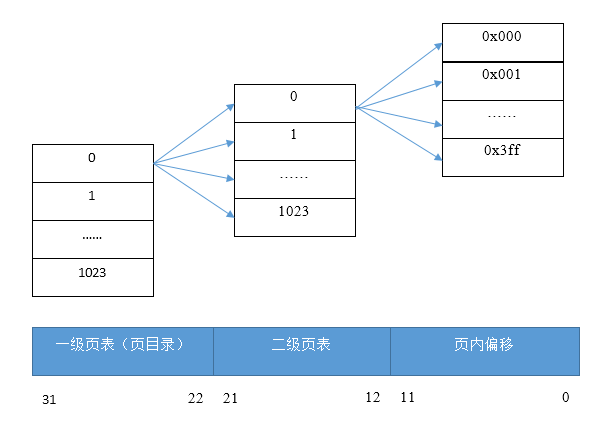
\includegraphics[width=12cm]{lab2-pic-1}
  \caption{二级页表结构示意图}\label{lab2-pic-1}
\end{figure}

第一级表称为页目录(page directory),一共1024个页目录项,每个页目录项32位(4 Byte),页目录项存储
的值为其对应的二级页表入口的物理地址。整个页目录存放在一个页面(4KB)中,也就是我们在 mips\_vm\_init
函数中为其分配了相应的物理内存。第二级表称为页表(page table),每一张页表有1024个页表项,每个页表
项32位(4 Byte),页表项存储的是对应页面的页框号(20位)以及标志位(12位)。每张页表占用一个页面大小
(4KB)的内存空间。

对于一个32位的虚存地址,其31-22位表示的是页目录项的索引,21-12位表示的是页表项的索引,11-0位表示的
是该地址在该页面内的偏移。

\subsection{地址转换}

对于操作系统来说,虚拟地址与物理地址之间的转换是内存管理中非常重要的内容。在这一部分,我们将详细探讨
咱们的内核是如何进行地址转换的。

首先从较为简单的形式开始。在前面的实验中,我们通过设置 lds 文件让操作系统内核加载到内存的 0x80010000
位置,在上文我们对 MIPS 存储器映射布局的介绍中我们知道,这一地址对应的是 kseg0 区域,这一部分的地址
转换不通过 MMU 进行。我们也称这一部分虚拟地址为内核虚拟地址。从虚拟地址到物理地址的转换只需要清掉
最高位的零即可,反过来,将对应范围内的物理地址转换到内核虚拟地址,也只需要将最高位设置为1即可。我们在
 include/mmu.h 中定义了 PADDR 和 KADDR 两个宏来实验这一功能:

\begin{minted}[linenos]{c}
// translates from kernel virtual address to physical address.
#define PADDR(kva)            \
  ({                \
    u_long a = (u_long) (kva);        \
    if (a < ULIM)         \
      panic("PADDR called with invalid kva %08lx", a);\
    a - ULIM;           \
  })

// translates from physical address to kernel virtual address.
#define KADDR(pa)           \
  ({                \
    u_long ppn = PPN(pa);         \
    if (ppn >= npage)         \
      panic("KADDR called with invalid pa %08lx", (u_long)pa);\
    (pa) + ULIM;          \
  })
\end{minted}

在 PADDR 中,我们使用了一个宏 ULIM ,这个宏定义在 include/mmu.h 中,其值为 0x80000000。对于小于
 0x80000000 的虚拟地址值,显然不可能是内核区域的虚拟地址。在 KADDR 中,一个合理的物理地址的物理
页框号显然不能大于我们在 mm/pmap.c 中所定义的物理内存总页数 npage 的值。

接下来,我们讨论如何通过二级页表进行虚拟地址到物理地址的转换。

首先,我们可以通过 PDX(va) 来获得一个虚拟地址对应的页目录索引,然后直接以凭借索引在页目录中得到对应的
二级页表的基址(物理地址),然后把这个物理地址转化为内核虚拟地址(KADDR),之后,通过 PTX(va) 获得这个
虚存地址对应的页表索引,然后就可以从页表中得到对应的页面的物理地址。整个转换的过程如 图\ref{lab2-pic-2}
所示:

\begin{figure}[htbp]
  \centering
  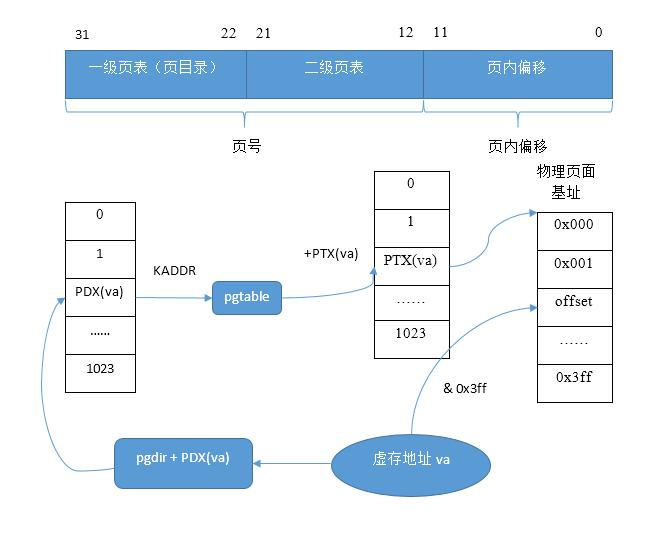
\includegraphics[width=12cm]{lab2-pic-2}
  \caption{地址转换过程}\label{lab2-pic-2}
\end{figure}

\subsection{页目录自映射}

上文中我们讲二级页表结构的时侯提到,要映射整个4G地址空间,一共需要1024个页表和1个页目录的。一个页表占用 4KB
空间,页目录也占用 4KB 空间,也就是说,整个二级页表结构将占用 4MB+4KB 的存储空间,1024*4KB+1*4KB=4MB+4KB。

在 include/mmu.h 中的内存布局图里有这样的内容:

\begin{minted}[linenos]{c}
/**
 *      ULIM     -----> +----------------------------+------------0x8000 0000-------
 *                      |         User VPT           |     PDMAP                /|\
 *      UVPT     -----> +----------------------------+------------0x7fc0 0000    |
 */
\end{minted}

不难计算出 UVPT(0x7fc00000) 到 ULIM(0x80000000) 之间的空间只有 4MB ,这一区域就是进程的
页表的位置,于是我们不禁想问:页目录所占用的 4KB 内存空间在哪儿?

\textbf{答案就在于页目录的自映射机制!}

如果页表和页目录没有被映射到进程的地址空间中,而一个进程的4GB地址空间又都映射了物理内存的话,那么就确实需要
1024个物理页(4MB)来存放页表,和另外1个物理页(4KB)来存放页目录,也就是需要(4M+4K)的物理内存。但是页表也被映射
到了进程的地址空间中,也就意味着 1024 个页表中,有一个页表所对应的 4M 空间正是这 1024 个页表所占用的 4M 内存,
这个页表的 1024 的页表项存储了 1024 个物理地址,分别是 1024 个页表的物理地址。而在二级页表结构中,页目录
对应着二级页表,1024 个页目录项存储的也是全部 1024 个页表的物理地址。也就是说,一个页表的内容和页目录的
内容是完全一样的,正是这种完全相同,使得将 1024 个页表加 1 个页目录映射到地址空间只需要 4M 的地址空间,
\textbf{其中的一个页表和页目录完全重合了}。

接下来我们会想到这样一个问题:那么,这个与页目录重合的页表,也就是页目录究竟在哪儿呢?

我们知道,这 4M 空间的起始位置也就是第一个二级页表对应着页目录的第一个页目录项,同时,由于 1M 个页表项和 4G
地址空间是线性映射,不难算出 0x7fc00000 这一地址对应的应该是第 (0x7fc00000 >> 12) 个页表项,这个页表项
也就是第一个页目录项。一个页表项 32 位,占用 4 个字节的内存,因此,其相对于页表起始地址 0x7fc000000 的
偏移为 (0x7fc00000 >> 12) * 4 = 0x1ff000 ,于是得到地址为 0x7fc00000 + 0x1ff000 = 0x7fdff000 。也就是
说,页目录的虚存地址为 0x7fdff000。

\begin{thinking}\label{think-windows_pde_addr}
了解了二级页表页目录自映射的原理之后,我们知道,Win2k内核的虚存管理也是采用了二级页表的形式,其页表所占的 4M
空间对应的虚存起始地址为 0xC0000000,那么,它的页目录的起始地址是多少呢?
\end{thinking}

\subsection{创建页表}

将虚拟地址转换为物理地址的过程中,如果这个虚拟地址所对应的二级页表不存在,有时,我们可能需要为这个
虚拟地址创建一个新的页表。我们需要申请一页物理内存来存放这个页表,然后将他的物理地址赋值给对应的页
目录项,最后设置好页目录项的权限位即可。

我们的内核在 mm/pmap.c 中分定义了 boot\_pgdir\_walk 和 pgdir\_walk 两个函数来实现地址转换和
页表的创建,这两个函数的区别仅仅在于当虚存地址所对应的页表的页面不存在的时候,分配策略的不同和使用的
内存分配函数的不同。前者用于内核刚刚启动的时候,这一部分内存通常用于存放内存控制块和进程控制块等数据
结构,相关的页表和内存映射必须建立,否则操作系统内核无法正常执行后续的工作。然而用户程序的内存
申请却不是必须满足的,当可用的物理内存不足时,内存分配允许出现错误。boot\_pgdir\_walk 被调用时,
还没有建立起空闲链表来管理物理内存,因此,直接使用 alloc 函数以字节为单位进行物理内存的分配,而
 pgdir\_walk 则在空闲链表初始化之后发挥功能,因此,直接使用 page\_alloc 函数从空闲链表中
以页为单位进行内存的申请。

上文中介绍了页目录自映射的相关知识,我们了解到页目录其实也是一个页表。我们知道,在咱们实验使用的内核中,
一个页表指向的物理页面存在的标志是页表项存储的值的 PTE\_V 标志位被置为 1 。因此,在将页表的物理地址赋值
给 页目录项时,我们还为页目录项设置权限位。

\begin{exercise}
完成 mm/pmap.c 中的 boot\_pgdir\_walk 和 pgdir\_walk 函数,实现虚拟地址到物理地址的转换以及创建页表的功能。
\end{exercise}

\subsection{地址映射}
一个空荡荡的页表自然不会对我们的内存翻译有帮助,我们需要在具体的物理内存与虚拟地址间建立映射,即将相应的物理页面地址填入对应虚拟地址的页表项中。
\begin{exercise}
实现 mm/pmap.c 中的 boot\_map\_segment 函数,实现将制定的物理内存与虚拟内存建立起映射的功能。
\end{exercise}

\subsection{page insert and page remove}

\begin{minted}[linenos]{c}
// Overview:
//   Map the physical page 'pp' at virtual address 'va'.
//   The permissions (the low 12 bits) of the page table entry
//   should be set to 'perm|PTE_V'.
//
// Post-Condition:
//   Return 0 on success
//   Return -E_NO_MEM, if page table couldn't be allocated
//
// Hint:
//   If there is already a page mapped at `va`, call page_remove()
//   to release this mapping.The `pp_ref` should be incremented
//   if the insertion succeeds.
int
page_insert(Pde *pgdir, struct Page *pp, u_long va, u_int perm)
{
	u_int PERM;
	Pte *pgtable_entry;
	PERM = perm | PTE_V;

	/* Step 1: Get corresponding page table entry. */
	pgdir_walk(pgdir, va, 0, &pgtable_entry);

	if (pgtable_entry != 0 && (*pgtable_entry & PTE_V) != 0) {
		if (pa2page(*pgtable_entry) != pp) {
			page_remove(pgdir, va);
		}
		else{
			tlb_invalidate(pgdir, va);
			*pgtable_entry = (page2pa(pp) | PERM);
			return 0;
		}
	}

	/* Step 2: Update TLB. */
	tlb_invalidate(pgdir, va);

	/* Step 3: Do check, re-get page table entry to validate
	 *  the insertion. */
	if (pgdir_walk(pgdir, va, 1, &pgtable_entry) != 0) {
		return -E_NO_MEM;    // panic ("page insert failed .\n");
	}

	*pgtable_entry = (page2pa(pp) | PERM);
	pp->pp_ref++;
	return 0;
}
\end{minted}

这个函数虽然我们并没有填,但是\textbf{非常重要}!这个函数将在\textbf{lab3和lab4}中被反复用到,这个函数
将va虚拟地址和其要对应的物理页pp的映射关系以perm的权限设置加入页目录。我们大概讲一下函数的执行流程与执行要点。

\textbf{流程大致如下:}先判断va是否有对应的页表项:如果页表项有效(或者叫va是否已经有了映射的物理地址)
的话,则去判断这个物理地址是不是我们要插入的那个物理地址,如果不是,那么就把该物理地址移除掉;
如果是的话,则修改权限,放到tlb中。

\textbf{有一个值得指出的要点}:我们能看到,只要对页表的内容修改,都必须tlb\_invalidate 来让tlb更新,否则后面紧接着对内存的访问很有可能出错。

可以说tlb\_invalidate 函数是它的一个核心子函数,这个函数实际上又是由tlb\_out 汇编函数组成的。

\begin{codeBoxWithCaption}{TLB汇编函数\label{code:tlb_out.S}}
  \inputminted[linenos]{gas}{codes/tlb_out.S}
\end{codeBoxWithCaption}

这个汇编函数相对其他汇编函数来说相对简单,那么留给你一个思考问题.

\begin{thinking}\label{think-tlb}
思考一下tlb\_out 汇编函数,结合代码阐述一下跳转到\textbf{NOFOUND}的流程?
\end{thinking}
\subsection{访存与TLB重填}
  通过之前的实验,我们可以知道,虚拟地址通过MMU转换成物理地址,然后通过物理地址我们能够在主存中获得相应的数据。而实际上,在MIPS架构中,关于这一块
  内存翻译的内容,很大程度上与TLB有关。TLB可以看做是一块页表的高速缓存,里面存储了一些物理页面与虚拟页面的对应关系。而当CPU访问相应内存地址时,会先去
  TLB中查询。当TLB中没有相应对应关系时会触发一个\textbf{TLB缺失异常}。而而MIPS将这个异常的处理,全权交给了软件。因此若发生缺失异常,则会跳转到相应异常处理程序中,
  再由我们的二级页表进行相应的地址翻译,对TLB进行重填。换句话说,MIPS中并没有一个执行内存地址翻译的MMU处理器,CPU完成了相应工作。

  为了深究整个过程,我们需要设置好相应的链接脚本,使得mips的异常处理机制能够正常工作(关于此处和异常的详情请参照lab3中相关内容)

  接着我们在page\_check最后一句printf之前添加如下代码段。
  \begin{minted}[linenos]{c}
    u_long* va = 0x12450;
    u_long* pa;

    page_insert(boot_pgdir, pp, va, PTE_R);
    pa = va2pa(boot_pgdir, va);
    printf("va: \%x -> pa: \%x\\n", va, pa);
    *va = 0x88888;
    printf("va value: \%x\\n", *va);
    printf("pa value: \%x\\n", *((u_long *)((u_long)pa + (u_long)ULIM)));
  \end{minted}

  这段代码旨在计算出相应va与pa的对应关系,设置权限位为PTE\_R是为了能够将数据写入内存。
  \begin{thinking}\label{think-memory-access}
  显然,运行后结果与我们预期的不符,va值为0x88888,相应的pa中的值为0。这说明我们的代码中存在问题,请你仔细思考我们的访存模型,指出问题所在。
  \end{thinking}
  \begin{thinking}\label{think-tlb-refill}
  在gxemul中,通过添加-t参数能够看到镜像中函数调用关系,请你善加利用这个特性,找出与tlb重填有关的函数。
  \end{thinking}
  另外,还可以提醒大家的是,在gxemul中,有tlbdump这个命令,可以随时查看tlb中的内容。
\section{正确结果展示}

实验二做完之后,正确的结果应该是这样的:

\begin{minted}[linenos]{c}
main.c: main is start ...
init.c: mips_init() is called
Physical memory: 65536K available, base = 65536K, extended = 0K
to memory 80401000 for struct page directory.
to memory 80431000 for struct Pages.
mips_vm_init:boot_pgdir is 80400000
pmap.c:  mips vm init success
start page_insert
va2pa(boot_pgdir, 0x0) is 3ffe000
page2pa(pp1) is 3ffe000
pp2->pp_ref 0
end page_insert
page_check() succeeded!
panic at init.c:55: ^^^^^^^^^^^^^^^^^^^^^^^^^^^^^^^^^^^^^
\end{minted}

最后一行的数字 \textbf{55} 是不固定的。

\section{实验思考}

\begin{itemize}
\item \hyperref[think-do_while]{\textbf{\textcolor{baseB}{思考-使用do-while(0)语句的好处}}}
\item \hyperref[think-bzero]{\textbf{\textcolor{baseB}{思考-bzero参数探究}}}
\item \hyperref[think-windows_pde_addr]{\textbf{\textcolor{baseB}{思考-自映射机制页目录地址的计算}}}
\item \hyperref[think-tlb]{\textbf{\textcolor{baseB}{思考-NOFOUND的奥妙}}}
\item \hyperref[think-memory-access]{\textbf{\textcolor{baseB}{思考-访存的问题}}}
\item \hyperref[think-tlb-refill]{\textbf{\textcolor{baseB}{思考-寻找重填函数}}}
\end{itemize}

\section{挑战性任务}

我们的虚存管理系统分配和回收页面粒度的内存,问题是如果我们需要支持真正的I/O设备,需要分配超过4KB的物理连续的内存;如果我们需要用户态使用,为了提高CPU效率,我们需要分配大小超过4MB的超级页。修改虚存管理,使得可以一次申请2的指数大小的内存,你可以自行设置大小的上限。确保,在需要的时候,将大的存储单元分为小的存储单元;如果可能,将小的存储单元合并为大的存储单元。
